\documentclass{standalone}
\usepackage{tikz,pgfplots}
\usepackage{newtxmath}

% definitions for interference images
\colorlet{wall}{blue!30!black}
\colorlet{myblue}{blue!70!black}
\colorlet{myorange}{orange!90!black!80}
\colorlet{myred}{red!70!black}
\colorlet{mydarkred}{red!50!black}
\colorlet{mylightgreen}{green!60!black!70}
\colorlet{mygreen}{green!60!black}
\colorlet{myredgrey}{red!50!black!80}
\colorlet{myshadow}{blue!30!black!90}
\tikzstyle{wave}=[myblue,thick]

\begin{document}

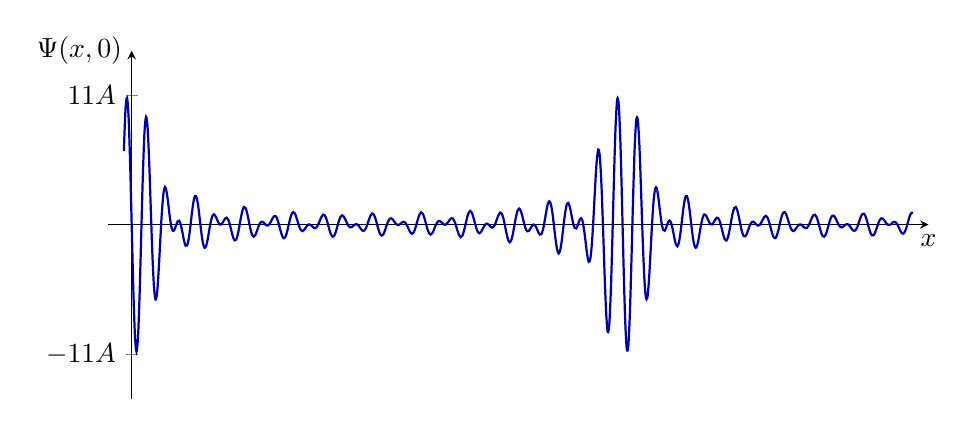
\begin{tikzpicture}
        \begin{axis}[xtick=\empty,
                    ytick={-11,11},
                    yticklabels={$-11A$,$11A$},
                    axis lines=middle,
                    enlarge x limits={abs=2},
                    enlarge y limits={abs=4},
                    x label style={anchor=north},
                    y label style={anchor=east},
                    xlabel={$x$},
                    ylabel={$\Psi(x,0)$},
                    width=12cm,
                    height=6cm]
        \addplot[domain=-1:100,samples=500,smooth,myblue,thick] {sin(deg(-2*x))+sin(deg(-2.1*x))+sin(deg(-2.2*x))+sin(deg(-2.3*x))+sin(deg(-2.4*x))+sin(deg(-2.5*x))+sin(deg(-2.6*x))+sin(deg(-2.7*x))+sin(deg(-2.8*x))+sin(deg(-2.9*x))+sin(deg(-3.0*x))};
        \end{axis}
    \end{tikzpicture}

\end{document}